\begin{equation}
    \begin{gathered}
        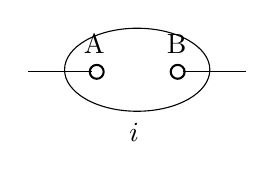
\begin{tikzpicture}[x=0.75pt,y=0.75pt,yscale=-1,xscale=1]
            %uncomment if require: \path (0,300); %set diagram left start at 0, and has height of 300
            
            %Straight Lines [id:da9495322085331372] 
            \draw    (88.5,105) -- (119.15,105) ;
            \draw [shift={(121.5,105)}, rotate = 0] [color={rgb, 255:red, 0; green, 0; blue, 0 }  ][line width=0.75]      (0, 0) circle [x radius= 3.35, y radius= 3.35]   ;
            %Straight Lines [id:da018779805704167263] 
            \draw    (162.85,105) -- (193.5,105) ;
            \draw [shift={(160.5,105)}, rotate = 0] [color={rgb, 255:red, 0; green, 0; blue, 0 }  ][line width=0.75]      (0, 0) circle [x radius= 3.35, y radius= 3.35]   ;
            %Shape: Ellipse [id:dp6737778885888006] 
            \draw   (106,104) .. controls (106,92.95) and (121.67,84) .. (141,84) .. controls (160.33,84) and (176,92.95) .. (176,104) .. controls (176,115.05) and (160.33,124) .. (141,124) .. controls (121.67,124) and (106,115.05) .. (106,104) -- cycle ;
            
            % Text Node
            \draw (136,128.4) node [anchor=north west][inner sep=0.75pt]    {$i$};
            % Text Node
            \draw (114,86) node [anchor=north west][inner sep=0.75pt]   [align=left] {A};
            % Text Node
            \draw (154,86) node [anchor=north west][inner sep=0.75pt]   [align=left] {B};
            \end{tikzpicture} 
    \end{gathered} = P = \dyad{+}{\uparrow \uparrow} + \dyad{-}{\downarrow \downarrow} + \frac{1}{\sqrt{2}} \ket*{0} (\bra*{\uparrow \downarrow} + \bra*{\downarrow \uparrow}).
    \label{eq:aklt-projector}
\end{equation}